\documentclass[a4paper]{article}
\usepackage{listings}
\usepackage{xcolor}
\usepackage {fontspec}
\setromanfont{Lantinghei SC Extralight}
\setmonofont{Courier New}
\XeTeXlinebreaklocale ``zh''
\XeTeXlinebreakskip = 0pt plus 1pt
\textheight = 650pt
\lstset{
	%行号
   numbers=left,
  %背景框
   framexleftmargin=10mm,
   frame=none,
   %背景色
   %backgroundcolor=\color[rgb]{1,1,0.76},
   backgroundcolor=\color[RGB]{245,245,244},
   %样式
   keywordstyle=\bf\color{blue},
   identifierstyle=\bf,
   numberstyle=\color[RGB]{0,192,192},
   commentstyle=\it\color[RGB]{0,96,96},
   stringstyle=\rmfamily\slshape\color[RGB]{128,0,0},
   %显示空格
   showstringspaces=false
 }

\begin{document}
\title{实验报告 实验五}
\author{姓名:王钦\quad 学号:13349112\quad 班级:计科二班}
\date{}

\maketitle
\section*{ 实验目的}
\hangindent=4em \hangafter=-10{
  1. 理解系统调用的实现方法。\\
  2. 实现原型操作系统中一些基本的系统调用。\\
  3. 设计并实现一测试系统调用的用户程序,利用系统调用实现用户界面和内部功能。\\
  4.在原型操作系统上建立一个初步C语言开发环境,理解操作系统与高级语言之间的关系。\\
}
\section*{ 实验内容}
\hangindent=4em \hangafter=-10{
在实验四的基础上,进化你的原型操作系统,增加下列操作系统功能:\\
(1)参考下面的系统调用功能表,增加一些其他功能\\
系统调用表(局部设计)\\
(2)扩展MYOS内核,实现上表中的所有(包括你增加的)系统调用,并开发一个用户程序,展示这些系统调用的使用效果。\\
(3)设计一个C程序库,封闭getch(),gets(),putch(),puts(),scanf()和printf()等利用系统调用实现的细节,并参考下面程序,开发一个用户程序,测试这些函数功能。\\

\begin{lstlisting}[language={C}]

include stdio.h
main(){
   	char ch,str[80];
   	int a;
   	getch(&ch);
   	gets(str);
   	scanf(“a=%d”,&a);
  	putch(ch);
  	puts(str);
   	printint(“ch=%c, a=%d, str=%s”, ch, a, str);
}
\end{lstlisting}

\section*{ 实验平台}
\hangindent=4em \hangafter=-10{
  gcc+nasm+Linux+vim\\
}

\section*{ 算法流程图}
\hangindent=4em \hangafter=-10{
  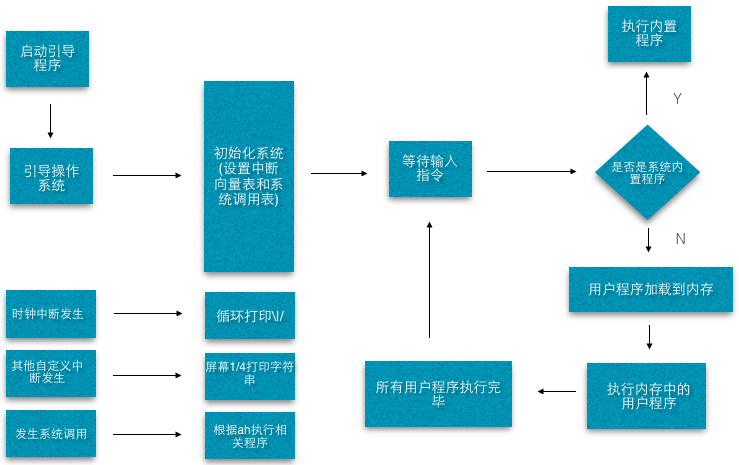
\includegraphics[scale=0.5]{Illustrations/flow.png}
}

\section*{ 实验步骤及效果}
\hangindent=4em \hangafter=-50{
1. 编辑修改ASM 文件,和C文件	\\\\
2. 使用make命令配合\verb|makefile|文件进行编译	\\\\
3. 运行\verb|bochs或vmware|虚拟机进行测试,进入后所看到的欢迎界面
{\center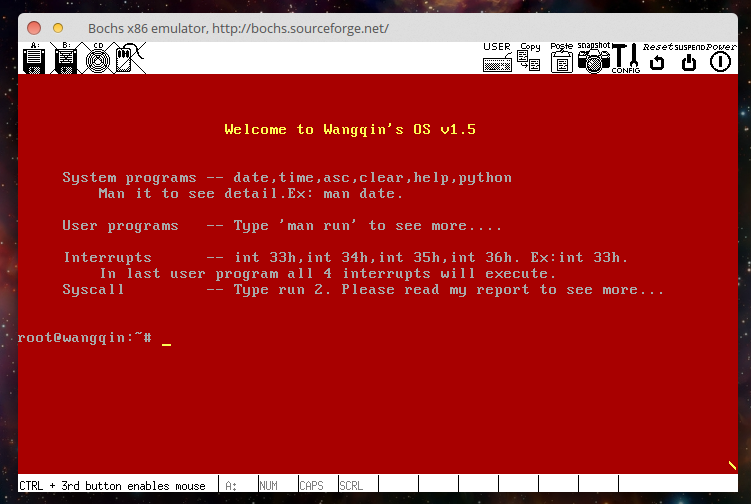
\includegraphics[scale=0.5]{Illustrations/start.png}}\\\\
4. 这次比实验三多了一个系统调用help.我们可以执行man help 查看这个调用的作用
{\center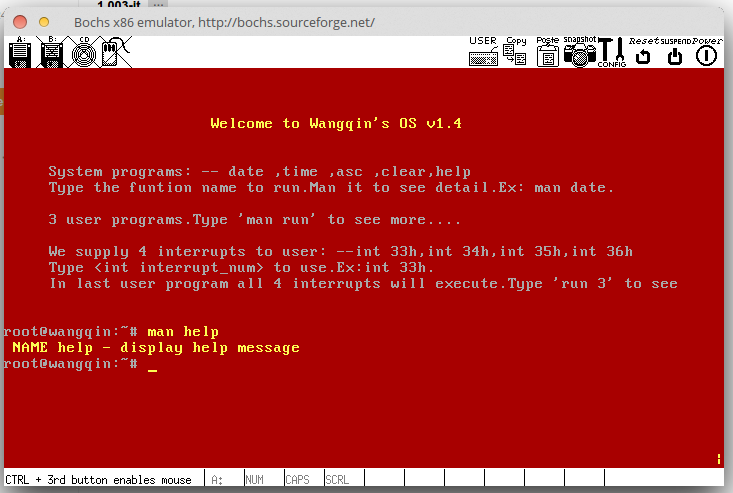
\includegraphics[scale=0.5]{Illustrations/manhelp.png}}\\\\
5. 输入int 33h,执行33h中断,可以看到左上角1/4屏幕打印出一个旋臂
{\center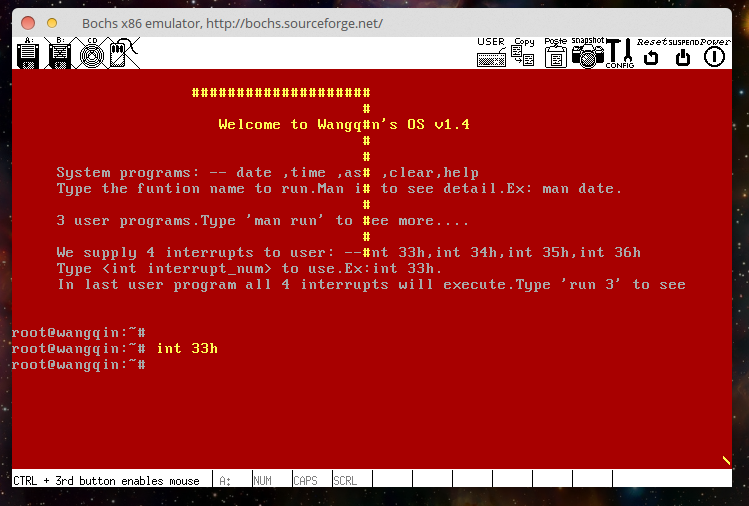
\includegraphics[scale=0.5]{Illustrations/int33h.png}}\\\\
6. 继续输入\verb|int 34h,int 35h,int 36h|,可以看到每次都在1/4屏幕上打印一个旋臂,直到生成了纳粹法西斯的标志:万字旗
{\center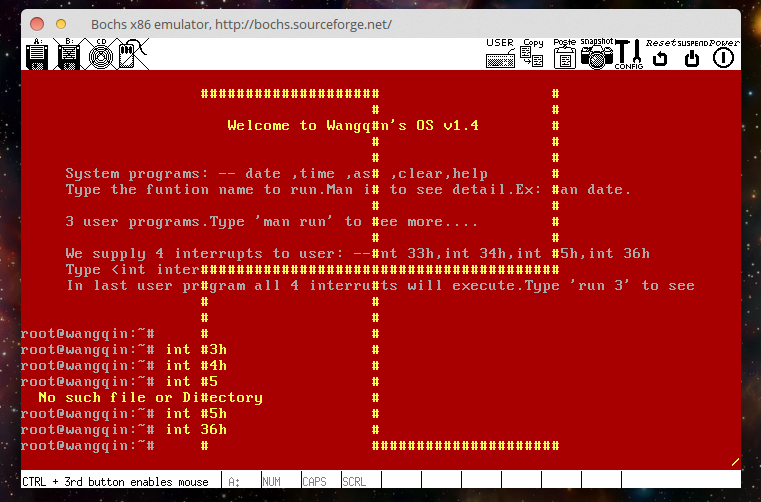
\includegraphics[scale=0.5]{Illustrations/allcustomint.png}}\\\\
7. 继续输入几个系统调用程序的名字,\verb|date time asc..|可以看到屏幕向上滚动,其实这个功能在上个实验已经实现
{\center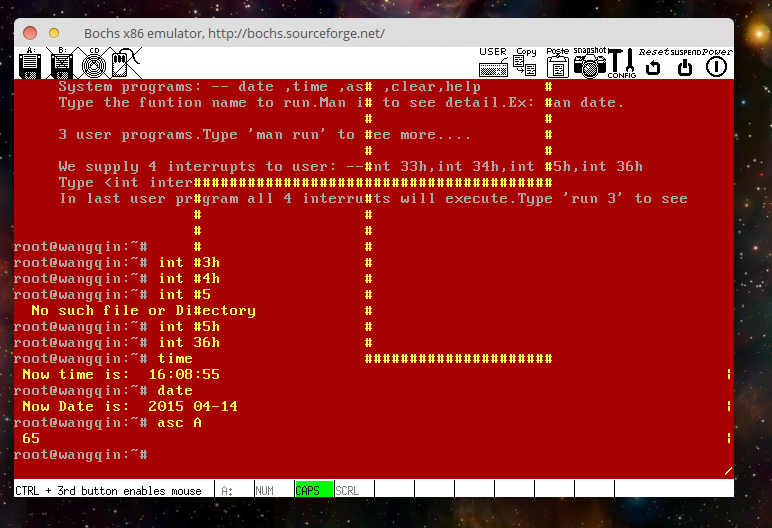
\includegraphics[scale=0.5]{Illustrations/syscall.png}}\\\\
8. 现在输入clear命令清除屏幕
{\center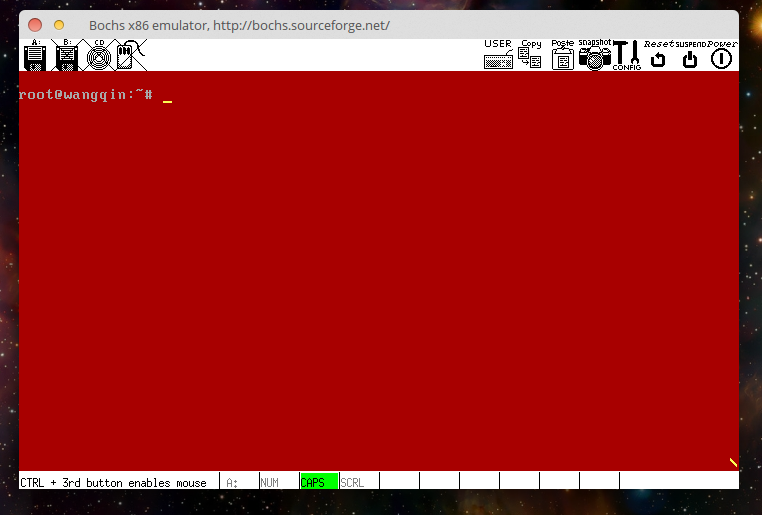
\includegraphics[scale=0.5]{Illustrations/afterclear.png}}\\\\
9. 输入run 语句来运行用户程序,一共有三个用户程序,一次run可以重复运行多个用户程序
{\center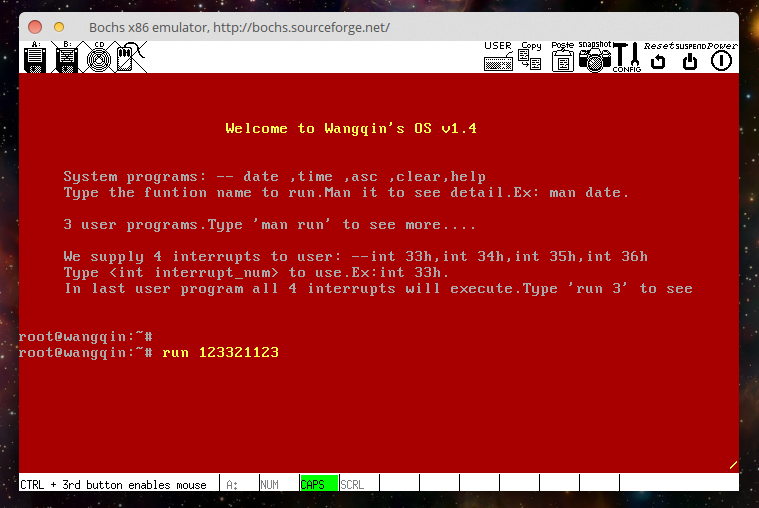
\includegraphics[scale=0.5]{Illustrations/runseqs.png}}\\\\
10. 进入用户程序之后键盘中断09h 就被重新修改了中断向量,只要检测到键盘敲击左上角就显示OACH。当敲击4次之后,此用户程序结束
{\center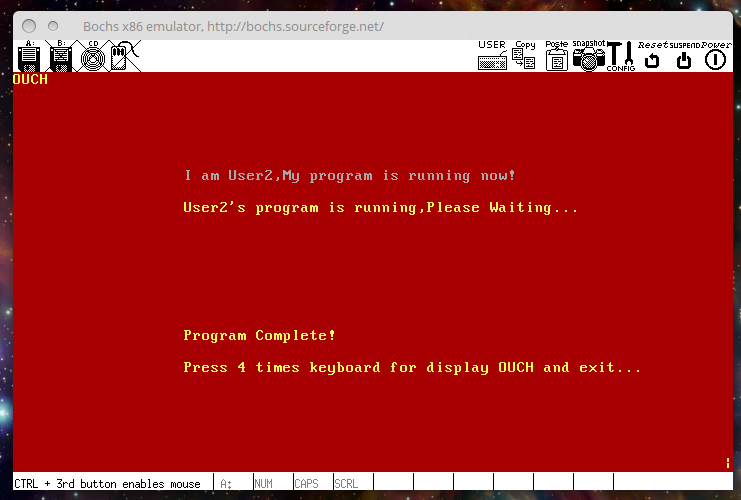
\includegraphics[scale=0.5]{Illustrations/ouch.png}}\\\\
11. 第3个用户程序,里面只有\verb|int 33h int 34h int 35h|这几条语句,可以看到其效果就是现实一个万字旗
{\center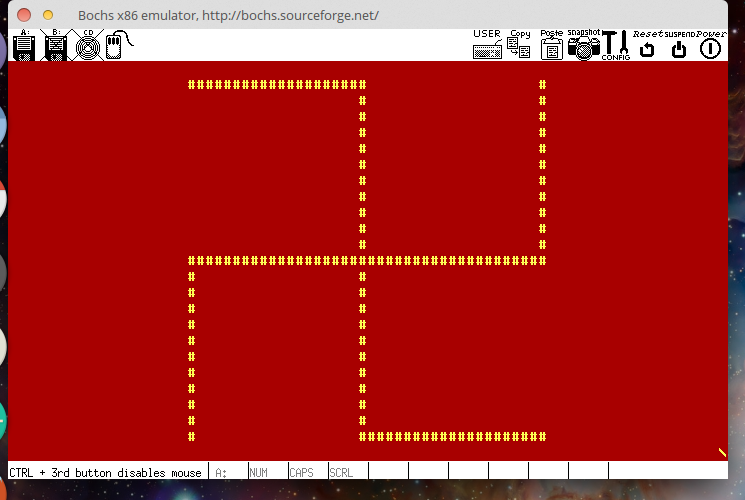
\includegraphics[scale=0.5]{Illustrations/usr3.png}}\\\\
12. 执行完所有用户程序之后,重新返回操作系统
{\center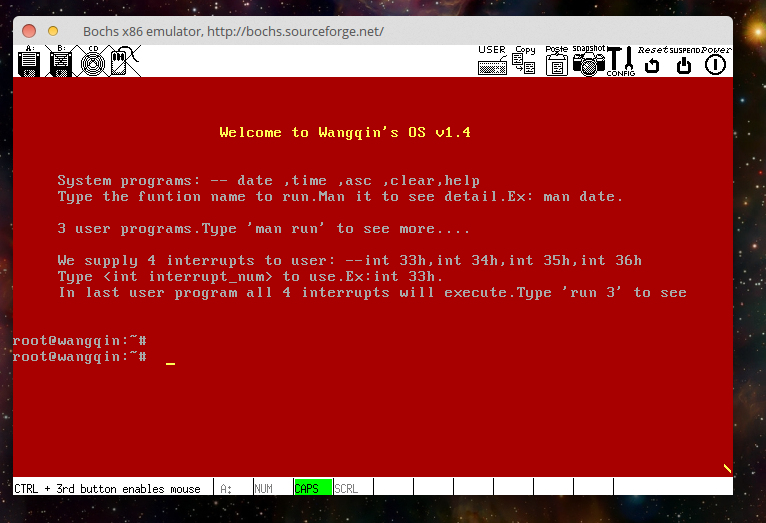
\includegraphics[scale=0.5]{Illustrations/backos.png}}\\\\
13. 在上述效果图中可以看到右下角始终有一个横杠在转动\\\\
}

\section*{ 内存和软盘存储管理}
\hangindent=4em \hangafter=-50{
1. 引导程序加载到内存0x7c00处运行\\
2. 引导程序将操作系统加载到0x7e00处运行\\
3. 操作系统讲用户程序加载到0x1000处运行\\
4. 软盘第1个扇区存储操作系统引导程序\\
5. 软盘第2~15扇区存储操作系统内核\\
6. 软盘第16~18扇区分别存储三个用户程序\\
}
\section*{ 主要函数模块解释}
\hangindent=4em \hangafter=-50{
	内核架构解释:os.c为内核主要控制模块,osclib.c os.asm主要为os.c提供函数实现.oslib.asm 为osclib.c提供更底层的函数封装\\\\
	1. \verb|os.c: main| 函数模块,这个在实验三报告中已经解释这里就不在赘述
	\begin{lstlisting}[language={C}]

 void main(){
     init_ss();
     screen_init();
     interrupt_init();
     print_welcome_msg();
     print_message();
     print_flag(); //root@wangqin4377@:   position

     while(1){
         char length = listen_key();

         unsigned short int now_row = get_pointer_pos()/256;
         if( now_row >23){       // 0~24   24 is deeplist line
             while( screen_sc_T--){
                 scroll_screen();
                 flag_scroll_up();
             }
         }

         flag_scroll();//move flag to next line
         print_flag();
     }
 }
	\end{lstlisting}
	2. 本次试验主要为了实现对中断向量表的修改工作,故在 os.asm中实现了下列函数为修改中断向量表提供调用
	\begin{lstlisting}[language={C}]
	;insert a interrupt vector
	insert_interrupt_vector:
	mov ax,0
	mov es,ax
	mov bx,[ interrupt_num]
	shl bx,2 ;interrupt num * 4 = entry
	mov ax,cs
	shl eax,8  ;shl 8 bit   *16
	mov ax,[ interrupt_vector_offset]
	mov [es:bx], eax
	ret
	\end{lstlisting}
	3. 要修改键盘中断的中断向量的时候,要考虑用户程序执行完了再把09h中断向量修改回去。所以要几个变量来保存之前09h指向的地址
	另外执行用户程序的时候用户press下key的时候,按下和抬起分别会触发09h中断故要开一个变量j来区分是按下还是抬起。i表示09中断被触发几次,达到4次即4*2=8则返回内核
	oslib.asm:
	\begin{lstlisting}[language={C}]

	var:
	i db 0      ;counter
	j db 0      ;reverse every time  0101
	flag db 0
	duan_1 dw 0
	offset_1 dw 0
	\end{lstlisting}
	4. 此为设置09h中断和执行用户程序的nasm代码
	\begin{lstlisting}[language={C}]
	run_user:
	push ecx
	push ax
	call screen_init

	;---------------------update 09 vector
	cli
	mov ax,0
	mov es,ax
	mov ecx,[ es:36]            ;backup
	mov [ duan_1],ecx

	mov ax,0x09
	mov [ interrupt_num], ax
	mov ax, key_detect
	mov [ interrupt_vector_offset],ax
	call insert_interrupt_vector
	mov ax,0
	mov [i],ax
	sti
	;--------------------run
	call 0x1000

	;--------------------reset 09 vector
	mov ax,0
	mov es,ax
	mov ecx,[ duan_1]
	mov [ es:36],ecx

	pop ax
	pop ecx
	ret
	\end{lstlisting}
	5. 系统初始化设置各个中断
	\begin{lstlisting}[language={C}]
	interrupt_init:
	mov ax,cs
	mov ds,ax

	;#1  setting up time interrupt
	mov ax,0x1c
	mov [ interrupt_num], ax
	mov ax, print_corner
	mov [ interrupt_vector_offset],ax
	call insert_interrupt_vector

	;#2 int 33
	mov ax,0x33
	mov [ interrupt_num], ax
	mov ax, process_int33
	mov [ interrupt_vector_offset],ax
	call insert_interrupt_vector

	;#3 int 34
	mov ax,0x34
	mov [ interrupt_num], ax
	mov ax, process_int34
	mov [ interrupt_vector_offset],ax
	call insert_interrupt_vector

	;#4 int 35
	mov ax,0x35
	mov [ interrupt_num], ax
	mov ax, process_int35
	mov [ interrupt_vector_offset],ax
	call insert_interrupt_vector

	;#5 int 36
	mov ax,0x36
	mov [ interrupt_num], ax
	mov ax, process_int36
	mov [ interrupt_vector_offset],ax
	call insert_interrupt_vector

	ret
	\end{lstlisting}
	6. 循环打印’|’、’/’和’$\backslash$’
	\begin{lstlisting}[language={C}]
	print_corner:
	; \ / [
	  mov ax,cs
	  mov ds,ax
	  mov ax,0xb800
	  mov es,ax

	  mov dl,30
	  mov al,[ pointer]       ; alert:  must be al  dont ax
	  cmp al,dl
	  jne next_print_c
	  mov byte [ pointer], 0
	  jmp cotinue_corner

	  next_print_c:
	  mov eax, cornerstring
	  mov ebx,0
	  mov bl,[ pointer]           ;ebx is added sum
	  add eax,ebx
	  mov al,[ eax]

	  inc ebx
	  mov [ pointer],bl

	  mov bx,3998D
	  mov [ es:bx],al

	  cotinue_corner:
	  iret

	  var:
	  flag_position dd 0x1000							;滚屏相关
	  interrupt_num dw 0x1c               ;init		
	  interrupt_vector_offset dw 0x7c00   ;init
	  pointer db 0
	  cornerstring db '\\\\\\\\\\||||||||||//////////'		;要循环打印的字符
	  ;int_user_num db 0


	\end{lstlisting}

	7. 显示OACH
	\begin{lstlisting}[language={C}]
	key_detect:
	cli
	push ax
	push bx
	mov ax,0xb800
	mov es,ax

	in al,60h
	in al,61h
	or al,80h
	out 61h,al
	mov al,61h
	out 20h,al

	mov bl,0
	mov bh,[j]
	cmp bl,bh
	je change1

	mov bh,0
	mov [j],bh
	mov byte [es:00],'O'
	mov byte [es:02],'U'
	mov byte [es:04],'C'
	mov byte [es:06],'H'

	jmp next_de

	change1:
	mov bh,1
	mov [j],bh

	mov byte [es:00],' '
	mov byte [es:02],' '
	mov byte [es:04],' '
	mov byte [es:06],' '

	next_de:

	mov bl,[i]
	inc bl
	mov [i],bl
	mov bh,8        ;press key 8 times
	cmp bh,bl
	jle closesti
	jmp niret
	closesti:
	mov cl,'A'

	niret:

	pop bx
	pop ax
	sti
	iret
	\end{lstlisting}
}

\section*{ 实验心得及仍需改进之处}
\hangindent=4em \hangafter=-50{
    实验心得:\\\\
\indent	通过本次实验我了解了x86架构下中断的机制和原理,通过手动编写中断处理程序和修改添加中断向量表中的中断向量实现了本实验的所有要求。
	在时钟中断的模块,刚开始打算改写08h的中断向量,后来经过网上查阅资料得知硬件中断08h会自动触发中断号为1ch的时钟中断,又叫\verb|time-tick|中断。
	通过改写1ch的中断处理程序即可实现时钟中断效果。\\ \indent 在后来的实验过程中发现有的用户程序无法读入内存,经过一番调试之后才发现自己操作系统太过庞大
	占用了15个扇区,加上四个用户程序和一个引导扇区共需要19个扇区,我只好减少了一个用户程序。并且把
	所有内联函数改为函数调用。最后只放了三个用户程序(其中最后一个将自动执行自定义的\verb|int 33,int 34, int 35, 36|中断)。估计在后面的试验中会不断的丰富操作系统的功能,
	目前我存储操作系统的
	15个扇区已经有14个被写满,下次实验考虑优化操作系统的代码使其短小精悍。\\ \indent 在后来在编写键盘中断处理程序的过程中,在
	编写中断向量号为09h的中断处理程序时由于不了解键盘中断的工作方式,明明写好了中断处理程序却只能第一次按键显示OUCH之后按键就不显示了。后来经过
	查阅相关资料发现还要对相关端口\verb|61h,60h,20h| 做一些处理才可以继续等待输入下个字符。\\\\
	实验仍需改进之处:\\\\
	仍需仔细检查多个中断发生的时候避免多个程序有无同时对同一个寄存器进行改写\\
	可以考虑增加文件系统\\
	没有加系统调用表\\
	考虑精简操作系统代码,减少冗余代码\\
	继续优化调整内核架构\\
}






\end{document}
